\section{Model - Exogenous Fertility}\label{sec:model1}

\begin{equation}
    \textbf{State space: }\statespace = \R^{2} \times \{0, 1, 2, 3, 4, 5\} \times \{ 18, 19, \cdots, 70\}
\end{equation}

\begin{equation}
    \textbf{Action space: }\actionspace  = 46 \cdot \{0, 15, 25, 37, 45\} 
\end{equation}

\begin{equation}
    \textbf{States: }\{G, Z, K, Q\}, \qquad \textbf{Actions: } \{H\} 
\end{equation}

The model represents the labour supply of married women - and the effect of children. More precisely it models a woman who can accumulate human capital by supplying a desired number of working hours. The woman can with a certain probability in each period give birth to a child, where, the number of children influences the utility. The model presented here has 4 states: $G$ which represents human capital, $Z$ which represents the agent's idiosyncratic wage path, $K$ the number of kids in the household and $Q$ which evolves in a deterministic fashion and represents the age of the agent. The action the agent can take in each period is a discrete number of working hours $H$.

\begin{equation}
    \textbf{Variables: }\{S, W, Y, M, U, L\},  \qquad \textbf{Parameters: } \{\beta_L, \beta_Y, p_\psi, \sigma_\epsilon, \delta, \zeta, \omega, \alpha, \eta_G, \eta_{G^2}\}
\end{equation}


To elaborate the rest of the model variables: Equation \eqref{eq:utility_v1} specifies is the how the agent get utility, $U$. Following the formulation of \textcite{adda_career_2011}, dividing the utility into sub-utility functions, where each sub-utility function allows for curvature by specifying a constant relative risk-averse (CRRA) function for each sub-utility. Assuming the special case of $\ln(\cdot)$. $L$ is leisure and $Y$ is the total income of the household. The parameters $\beta_L, \beta_YK$ is the individual weighing of the different sub-utilities. Note that for identification I will restrict $\beta_Y= 1$.
Equation \eqref{eq:leissure_v1} specifies the leisure of the agent. Following \textcite{firestone_estimation_1988}, \textcite{thrane_men_2000} and \textcite{ekert-jaffe_time_2015} I assume that some of the time spent with kids can be considered work. I let $\omega=3.5$ be the time spent of extra house work pr. children each week. The weekly number of hours supplied is also subtracted from the total amount of leisure. The number of hours is aggregated to annual level subtracting 6 weeks for holiday. Equation \eqref{eq:wage_v1} specifies the total annual wage of a person, denoted $W$. Again 46 weeks is considered with salary level multiplied with number of hours supplied on the labour market. Equation \eqref{eq:salary_tilde_v1} denotes the hourly Salary $\tilde{S}$. The salary creating process follows a mincer equation, as described by \textcite{lemieux_mincer_2006}. The equation implies that $\log \tilde{S}$ is a function of some constant $\alpha$, and the human capital accumulated on the job. The actual hourly salary is given in equation \eqref{eq:salary_v1}. The hourly salary has a lower bound of $S_{min}=120$ danish kroner. and otherwise it's considered the sum of the idiosyncratic wage path $Z$ and the $\tilde{S}$ which is the salary earned as a function of human capital. The total income of the household $Y_t$ is described by equation \eqref{eq:total_salary_v1} represents the households total earnings, where $f^M(Q_t)$ is the earnings of the husband, $W$ is the wage of the women. $f^M$ is modelled non parametric using data from Danmarks Statistik Bank, and is assumed to be a perfectly deterministic income path of the husband.

The states of the agent evolves the following way: Equation \eqref{eq:age_v1} evolves in a deterministic fashion. Letting the age $Q_t$ increment one year each period. The fertility is modeled in \eqref{eq:fertility_v1}, where $K_t$ (the number of children in the household) evolves by with a certain probability and extra children is added. This probability is dependent on the age of the women $Q$. The probability is found using data from statistics Denmark. Equation \eqref{eq:idiosyncratic_wage_path_v1} explains the idiosyncratic wage path of the women, assumed to follow a random walk. The Human capital accumulates with a constant depreciation rate $\delta$, adding the number of working hours last period.

\begin{align}
    U_t(L_t, Y_t) &= \beta_L \ln(L_t + 1) + \beta_Y \ln(Y_t + 1) \label{eq:utility_v1}\\
    L_t(K_t, H_t) &= 46 \cdot ((24 \cdot 7) - \omega \cdot K_t  - H_t) \label{eq:leissure_v1}\\
    W_t(S_t, H_t) &= 46 \cdot S_t \cdot H_t \label{eq:wage_v1}\\
    \log \tilde{S}_t (G_t, Z_t) &= \alpha + \eta_G G_t + \eta_{G^2} G_t^2 \label{eq:salary_tilde_v1}\\
    S_t(\tilde{S}_t) &= \max(S_{min} , \tilde{S}_t  + Z_t)  \label{eq:salary_v1}\\
    Y_t(W_t, M_t) &= W_t + f^M(Q_t) \label{eq:total_salary_v1}\\
\end{align}


Law of Motion.

\begin{align}
    Q_{t+1}(Q_t) &= Q_t \label{eq:age_v1}\\
    K_{t+1}(K_t, Q_t)  &= K_{t} + \psi_t, \qquad \psi_t \mid Q_t \sim Bernoulli(p_\psi(Q_t)) \label{eq:fertility_v1} \\
    Z_{t+1}(Z_t) &= Z_t + \epsilon_t, \qquad \epsilon_t \sim \ndist(0, \sigma_\epsilon) \label{eq:idiosyncratic_wage_path_v1}\\
    G_{t+1}(G_t) &= G_t(1 - \delta) + H_t \\
\end{align}


%\begin{figure}
%    \centering
%    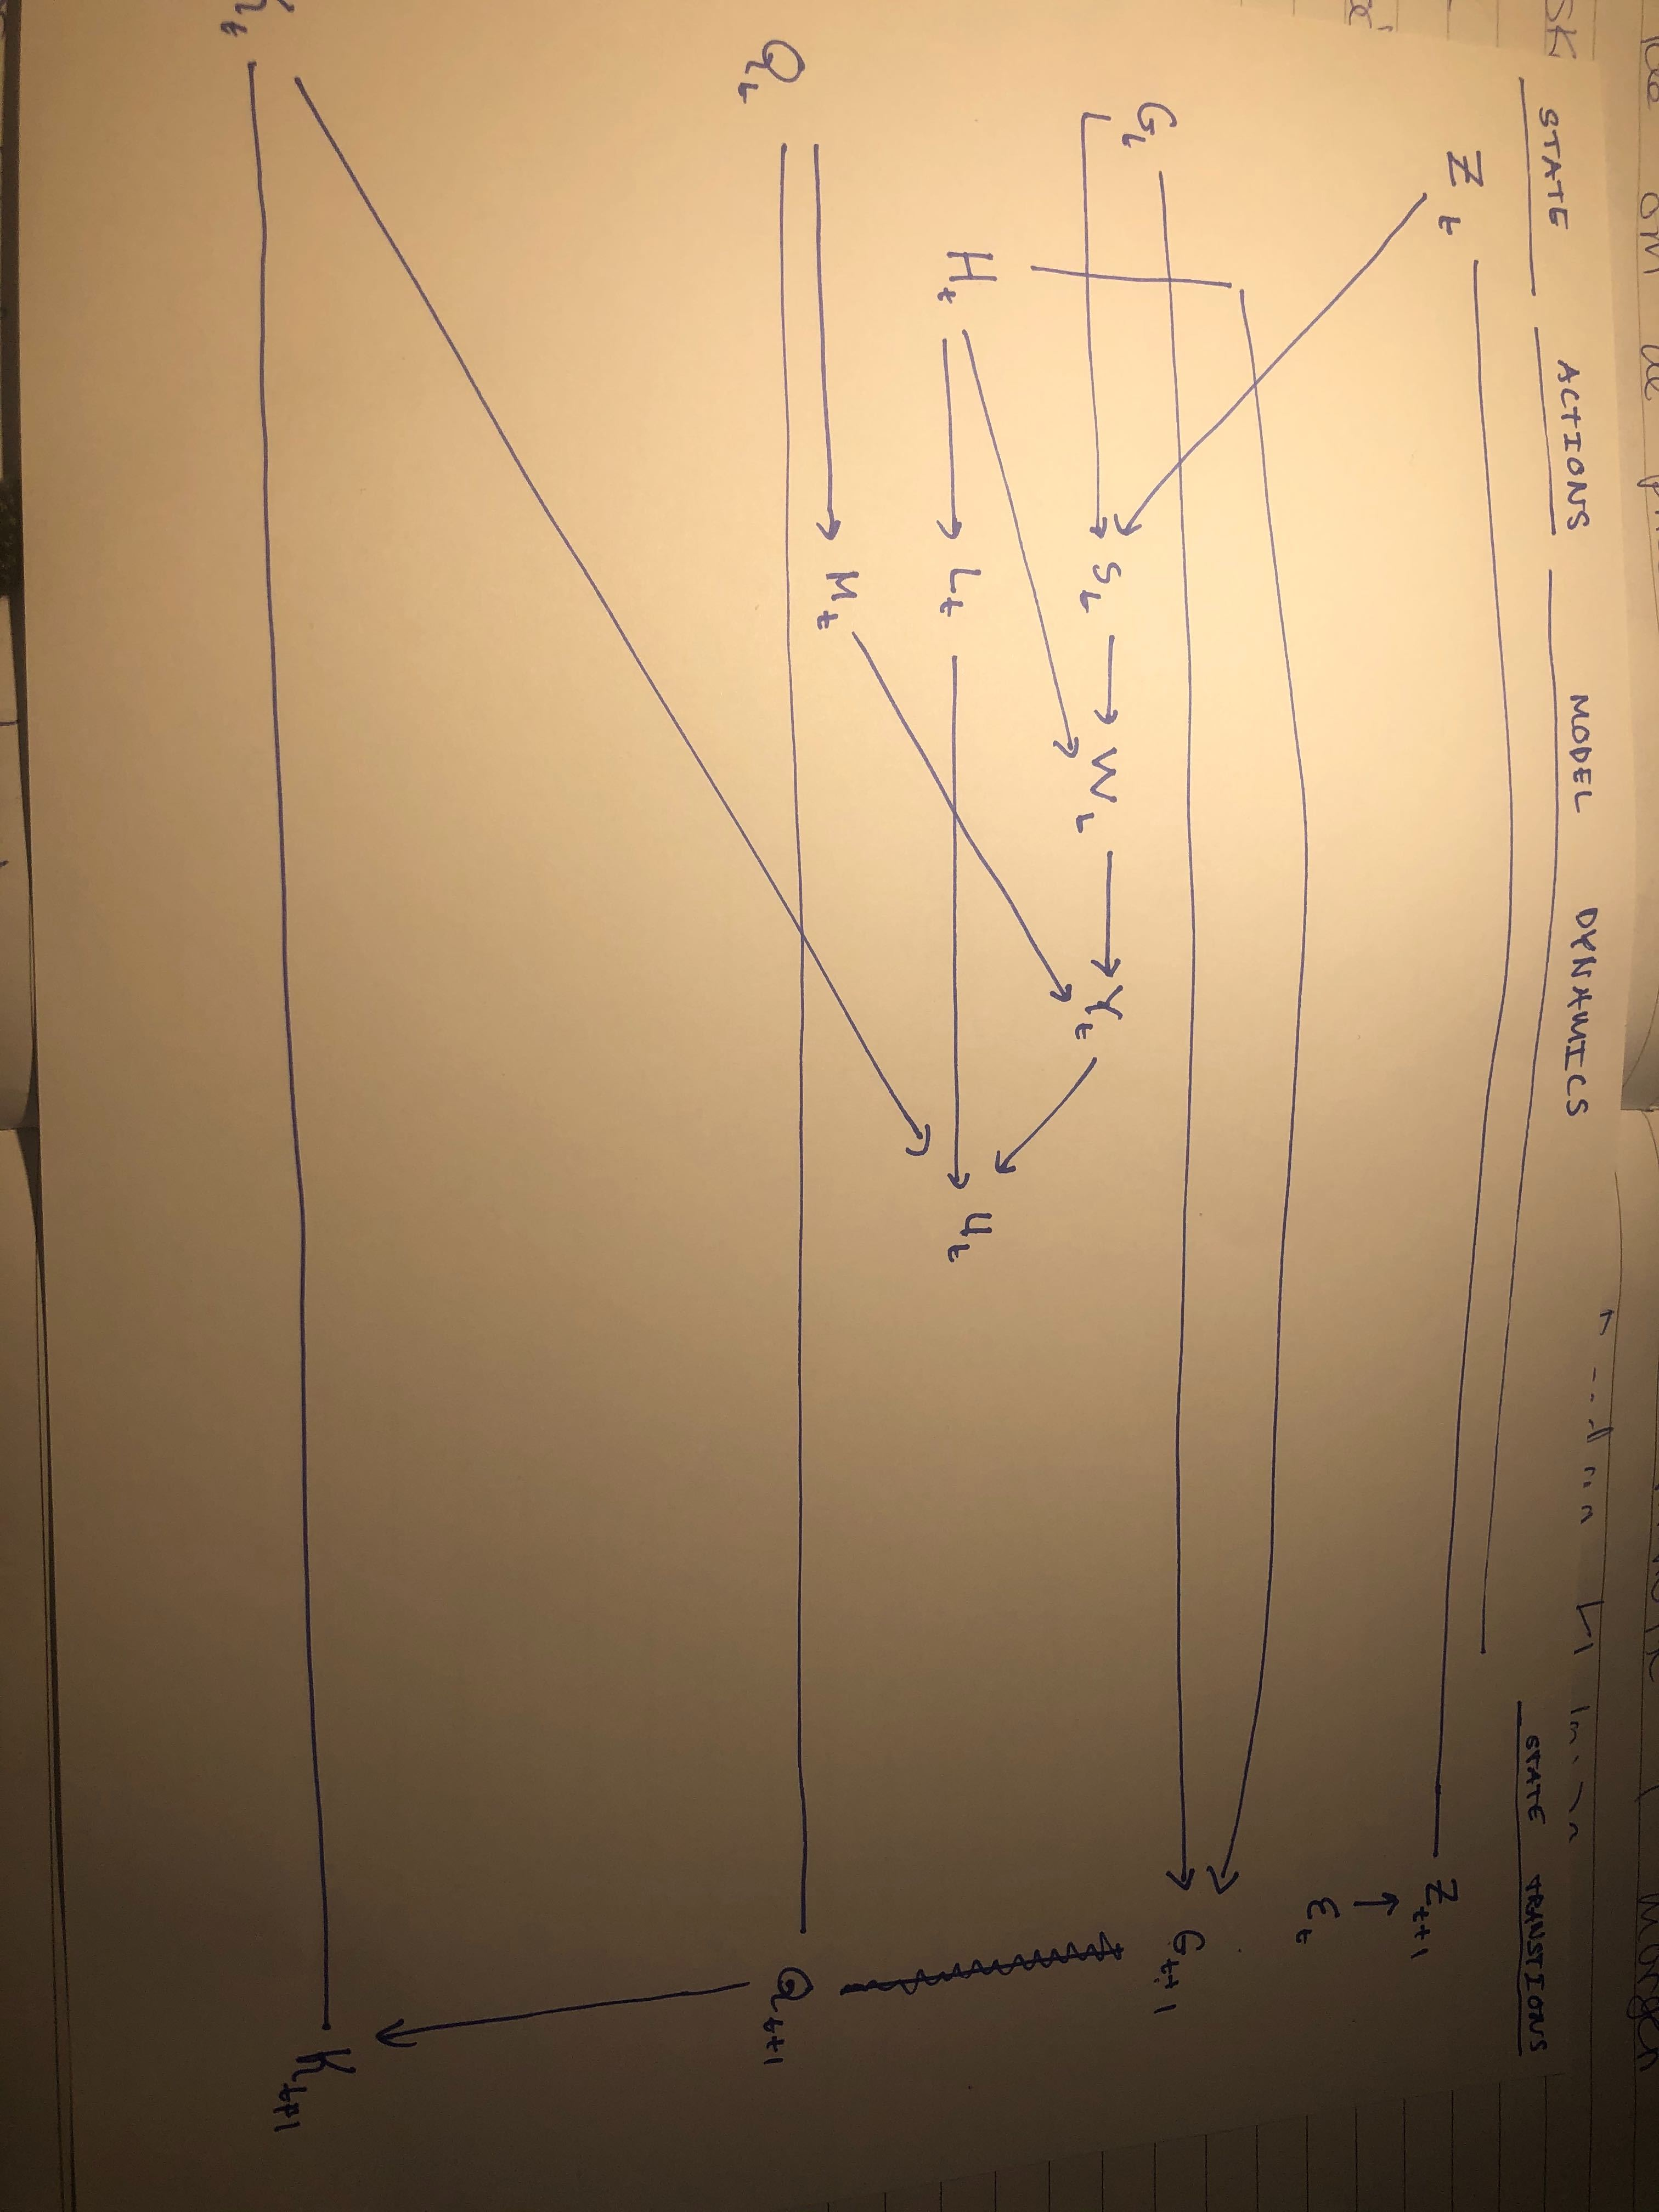
\includegraphics[scale=0.1, angle=90]{figures/modeldynamic_tmp_exogenous.jpg}
%    \caption{Model dynamics - Exogenous (TMP)}
%    \label{fig:tmp_modeldynamics_exogenous}
%\end{figure}